\documentclass{LU-nosleguma}


%par darbu
\title{Sabiedrības līdzdalības iespējas publiskajā pārvaldē Latvijā}
\thesistype{Bakalaura darbs}
%par autoru
\author{Pēteris Cinis}
\studentid{00010}
%par darba vadītāju
\supervisor{profesore Dr. polit. Inta Kalniņa}
%kur aizstāvēts
\university{Latvijas Universitāte}
\faculty{Datorikas fakultāte}
\location{Rīga}

\begin{document}
\maketitle
\setcounter{page}{2}
\pagestyle{empty}

\begin{abstract}
Anotāciju sagatavo divās valodās – latviešu un angļu valodā. Pēc saskaņošanas ar programmas 
direktoru var sagatavot arī papildu anotāciju kādā citā Eiropas Savienības oficiālajā valodā. 
Anotācijā izklāsta problēmas būtību, pētījuma mērķus, raksturo iegūtos rezultātus. 
Anotācijas apjoms ir noteikts līdz 850 zīmēm, ieskaitot intervālus.
\end{abstract}
\clearpage

%katra anotācija savā lapā.
\selectlanguage{english}
\begin{abstract}
An abstract is a brief summary of a research article, thesis, review, conference proceeding or any 
in-depth analysis of a particular subject or discipline, and is often used to help the reader quickly 
ascertain the paper's purpose. When used, an abstract always appears at the beginning of a 
manuscript or typescript, acting as the point-of-entry for any given academic paper or 
patent application. 
\end{abstract}
\clearpage

\pagestyle{plain}
\selectlanguage{latvian}


\tableofcontents


\section*{Ievads}
\addcontentsline{toc}{section}{Ievads}
Mūsdienās, kad ... \cite{darktome}


\section {Pirmā lielā nodaļa}
\subsection {Kolēģis Nr. 1}
Jā, godātie kolēģi! Runāsim par formu. Jā, tagad mēs apspriežam šo ļoti svarīgo jautājumu. Šodien Leiškalna kungs, 
aģitējot par šā lēmuma projekta iekļaušanu sēdes darba kārtībā, pateica, ka mums ir jālegalizē tas, kas jau ir noticis.

\subsection {Kolēģis Nr. 2}
Nu tad parunāsim par to, kas jau ir noticis! Tātad principā esam uzņēmušies saistības. Mums ir parlamentāra valsts.
Principā galīgais lēmums ir jāpieņem parlamentam, nevis valdībai. Taču iznāk tā, ka valdība uzņemas kādas saistības 
un pēc tam parlamentam jāpieņem viss, ko piedāvā valdība, jo tas ir iekļauts saistībās ar starptautiskajiem kreditoriem.

\section{Otrā lielā nodaļa}
Otrkārt. Ja uz laiku, kas nepārsniedz piecus gadus, viņš Latvijā iegādājas vienu vai vairākus īpašumus un šo darījumu
summa ir ne mazāka kā 100 tūkstoši latu Rīgā un Rīgas reģionā, bet, ja tas notiek ārpus Rīgas un ārpus Rīgas reģiona,
~--- ne mazāka kā 50 tūkstoši latu.

\subsection{Otrās nodaļas apakšnodaļa}
Un trešais nosacījums, kas varētu būt viens no veidiem. Ja uz laiku, kas nepārsniedz piecus gadus, veicis Latvijas 
kredītiestādē finanšu investīcijas~--- ne mazāk kā 200 tūkstošus latu~---, kuru termiņš ir ne mazāks par 5 gadiem, 
un ja noguldījuma noteikumi paredz, ka nav tiesību izbeigt pirms noguldījuma atmaksas termiņa.
Diemžēl šodien tehnisku iemeslu dēļ šie mūsu priekšlikumi tika atsaukti, bet Tautas partija un arī Tautsaimniecības, 
agrārās, vides un reģionālās politikas komisija noteikti sekos līdzi un atgriezīsies pie šiem priekšlikumiem uz trešo 
lasījumu.

\subsubsection{Otrās nodaļas apakš-apakšnodaļa}

\begin{figure}
	\centering
	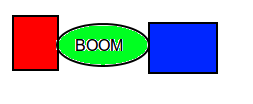
\includegraphics{maksla.png}
	\caption{Modernā māksla}
\end{figure}

\begin{table}
	\caption{Binārā reizināšanas tabula}
	\centering
	\begin{tabular}{r | l | l |}
		  & 0 & 1\\ \hline
		0 & 0 & 0\\ \hline
		1 & 0 & 1\\ \hline
	\end{tabular}
\end{table}

\bibliography{demo}
\bibliographystyle{plain}

\end{document}
